\section{Architecture and components}
\label{sec:arch}
The following chapter describes the individual components developed during this project as well as the interaction required between the components to fulfil the project goal of actuating the model car base on simulation data.
A diagram with the interactions between the components is visible in \autoref{fig:arch}.

The data from the SpeedDreams simulation is first received by the MQTT server on the \texttt{car-control} topic, as described in \autoref{sec:mqtt-car-control}.
The component running on the PandaBoard is subscribed to this MQTT topic and processes the information, see \autoref{sec:panda}.
The resulting commands are then published on the \texttt{car-servo} MQTT topic, described in \autoref{sec:mqtt-car-servo}.
The component running on the Raspberry Pi in turn is responsible for forwarding the commands according to the rules (\autoref{sec:rpi}) the commands to the Servo Control component (\autoref{sec:servo}).


\begin{figure}[h]
    \centering
    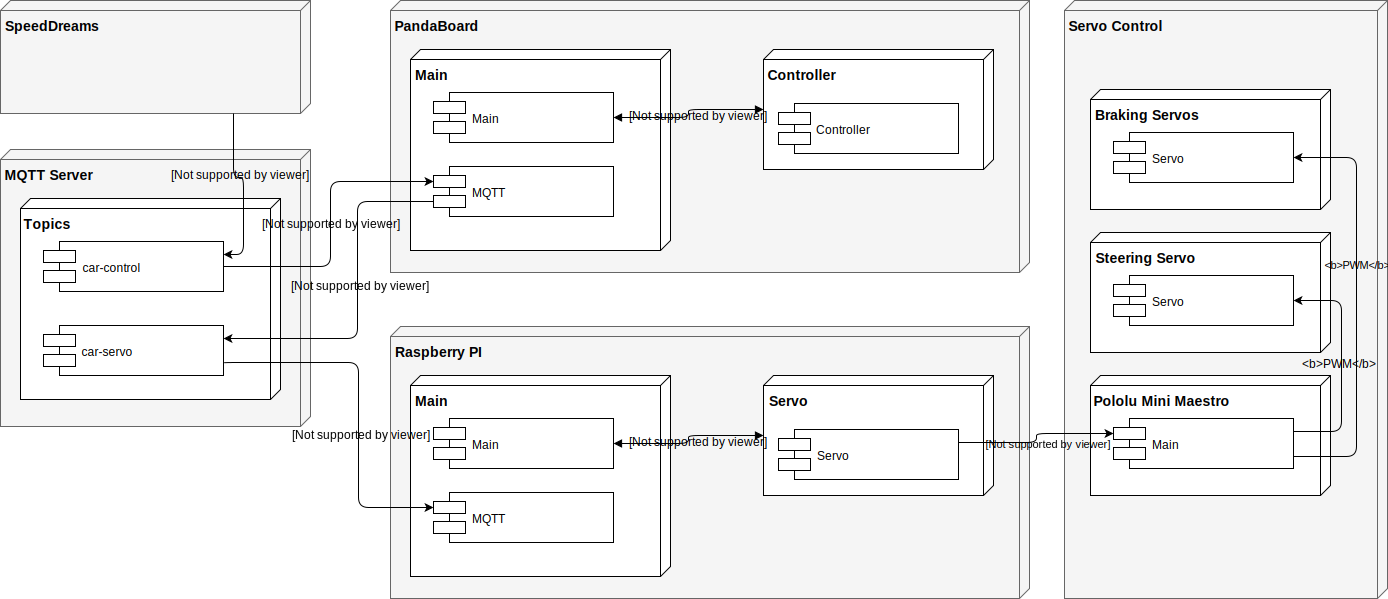
\includegraphics[width=1\linewidth]{images/components}
    \caption{Components overview}
    \label{fig:arch}
\end{figure}

\subsection{Servo (CG)}
\label{sec:servo}
%TODO CG Write chapter
\subsection{Raspberry Pi (TM)}
\label{sec:rpi}
%TODO TM Write chapter
\subsection{PandaBoard}
\label{sec:panda}
%TODO FM: Write chapter
